\documentclass[11pt,a4paper]{article}
\usepackage[utf8]{inputenc}\usepackage[margin=2.1cm]{geometry}
\usepackage{graphicx,booktabs,longtable,array,float,xcolor,enumitem,caption,fancyvrb}
\usepackage[hidelinks]{hyperref}\usepackage{url}
\captionsetup{font=small,labelfont=bf}\setlength{\parindent}{0pt}\setlength{\parskip}{4pt}
\setlist{itemsep=1pt,topsep=2pt}\setcounter{secnumdepth}{3}
\newcommand{\ph}[1]{\colorbox{yellow}{\textbf{[#1]}}}
\sloppy\emergencystretch=2em
\begin{document}
\begin{center}{\LARGE\bfseries 23CSE455 Design Patterns\\[2pt] Case Study Report}\end{center}
\textbf{Note.} Yellow boxes mark facts only the team can supply (team name, roll numbers, faculty approval, repository URL, screenshots, reviewer names). Everything else in this report was produced and checked from the supplied source code.
\medskip
{\small
\begin{center}\begin{tabular}{@{}p{3.3cm}p{12.4cm}@{}}
\toprule \textbf{Item} & \textbf{Content} \\ \midrule
Team & \ph{exact team name, team folder name: A15} \\
Case study & Design-pattern discovery, evolution and cross-language comparison of a Quarkus (Java) bank REST API; \ph{assigned domain/framework/title as given by the faculty} \\
Application & api-quarkus-2 (``REST API Bank - Quarkus''); faculty approval: \ph{name/date of approval} \\
Date & 2026-10-11 \\
Submission repository & \texttt{23CSE455\_\allowbreak{}DP\_\allowbreak{}CaseStudy}, team folder at the repository root \\
\bottomrule\end{tabular}\end{center}
}
{\small
\begin{center}\begin{tabular}{@{}p{4cm}p{6cm}p{5cm}@{}}
\toprule \textbf{Roll number} & \textbf{Student name} & \textbf{Batch} \\ \midrule
AM.AI.U4AID23009 & Hariprid V & AIDS \\
AM.AI.U4AID23017 & Pranav R Menon & AIDS \\
AM.AI.U4AID23022 & Sreyas A & AIDS \\
\bottomrule\end{tabular}\end{center}
}
\tableofcontents\newpage
\section{Application and architecture}
{\small
\begin{center}\begin{tabular}{@{}p{3cm}p{12.7cm}@{}}
\toprule \textbf{Item} & \textbf{Content} \\ \midrule
Original source & Repository URL: \texttt{https:\allowbreak{}/\allowbreak{}/\allowbreak{}github.\allowbreak{}com/\allowbreak{}dev-MichaelCruz/\allowbreak{}api-quarkus}; supplied as the archive \texttt{api-quarkus-main.\allowbreak{}zip} (no tag or version string inside). Baseline commit: \texttt{baa96db} = local import commit of the archive; the only edit is that the plain-text database password in \texttt{application.\allowbreak{}properties} was replaced by \texttt{\$\{DB\_\allowbreak{}PASSWORD:\allowbreak{}change-me\}} (never upload credentials). Access date 2026-10-11. License: none stated (no LICENSE file in the archive). \\
Environment & Project: Java release 17, Quarkus platform 3.6.1 (extensions: arc, hibernate-orm, hibernate-validator, resteasy-jackson, jdbc-mysql; junit5 and rest-assured for tests), MySQL. Working container: OpenJDK 21.0.12.1, Python 3.13.16, Node.js 22.22.0, g++ 13.3.0, lizard 1.24.1, Graphviz 2.43.0, pdfTeX 2023. \\
Scope & Inspected: all 17 production Java files (613 lines), \texttt{application.\allowbreak{}properties}, \texttt{pom.\allowbreak{}xml}. Excluded: Dockerfiles and \texttt{index.\allowbreak{}html} (no application logic), Maven wrapper scripts (tooling), and the template tests \texttt{GreetingResourceTest/\allowbreak{}IT} (they request \texttt{/\allowbreak{}hello}, which does not exist in \texttt{src/\allowbreak{}main}, so by inspection they cannot pass; removed in commit \texttt{c9d7097}). \\
Run instructions & README: \texttt{data/\allowbreak{}code/\allowbreak{}README.\allowbreak{}md} (project) and \texttt{data/\allowbreak{}code/\allowbreak{}api-quarkus-2/\allowbreak{}README.\allowbreak{}md}: \texttt{.\allowbreak{}/\allowbreak{}mvnw compile quarkus:\allowbreak{}dev} with a MySQL database configured through \texttt{DB\_\allowbreak{}PASSWORD}. \textbf{Actual result: not run.} Maven Central is unreachable from the working environment (proxy answers HTTP 403 to CONNECT), so no Quarkus build, \texttt{mvn test} or database run was possible. Substitute actually run: sandbox harness (real production sources compiled against Jakarta API stubs, in-memory EntityManager): \texttt{bash data/\allowbreak{}test\_\allowbreak{}result/\allowbreak{}harness/\allowbreak{}run\_\allowbreak{}tests.\allowbreak{}sh} -- 15/15 characterization tests passed on the unchanged baseline production code. \\
\bottomrule\end{tabular}\end{center}
}
\subsection{Architecture}
\begin{figure}[H]\centering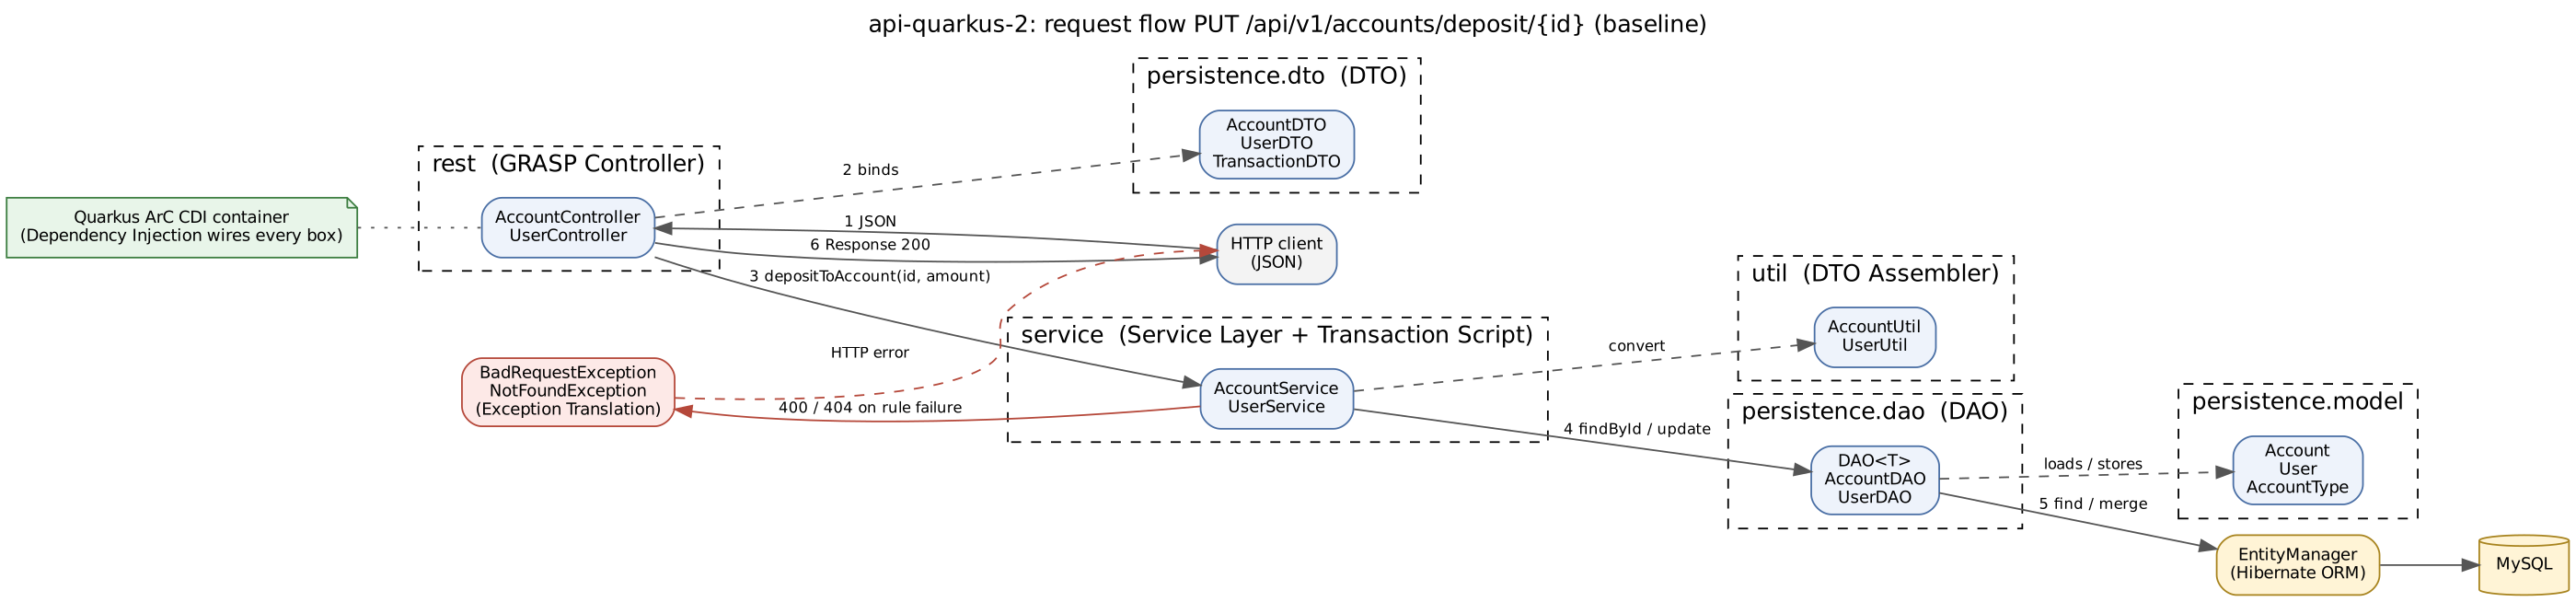
\includegraphics[width=0.92\linewidth]{Part1/pattern_architecture/architecture.png}\caption{Layered architecture and the request flow of PUT /api/v1/accounts/deposit/\{id\} (baseline). Source: Part1/pattern\_architecture/architecture.dot.}\end{figure}
The application is a classic layered REST service. \textbf{Components:} controllers (\texttt{rest}) bind JSON to DTOs and delegate; services (\texttt{service}) hold the use cases and the business rules; converters (\texttt{util}) map DTO and entity; DAOs (\texttt{persistence.\allowbreak{}dao}) wrap the JPA \texttt{EntityManager}; entities and DTOs live in \texttt{persistence.\allowbreak{}model} and \texttt{persistence.\allowbreak{}dto}; two \texttt{WebApplicationException} subclasses carry HTTP errors; the CDI container wires everything with \texttt{@Inject}.
\textbf{Request flow (deposit):} (1) the client sends JSON; (2) RESTEasy binds it to \texttt{TransactionDTO} and calls \texttt{AccountController.\allowbreak{}depositToAccount}; (3) the controller unwraps the amount and calls \texttt{AccountService.\allowbreak{}depositToAccount}; (4) the service loads the account through \texttt{AccountDAO.\allowbreak{}findById} (404 if absent), checks the amount, applies the savings bonus, and saves through \texttt{AccountDAO.\allowbreak{}update}; (5) the DAO calls \texttt{entityManager.\allowbreak{}merge}; (6) the controller answers 200. A rule violation throws \texttt{BadRequestException} (HTTP 400) which the JAX-RS runtime turns into the response.
\section{Part 1: Pattern discovery}
\textbf{Method.} Each member ran a prompt restricted to one layer (presentation/contract, business, persistence; files \texttt{Part1/\allowbreak{}Part1\textbackslash{}\_\allowbreak{}prompt.\allowbreak{}txt}, \texttt{Part1/\allowbreak{}llm/\allowbreak{}}) over the numbered baseline source. The team merged the three outputs, removed duplicates (the DTO and its assembler were seen from two sides) and decided rejections. \textbf{Source evidence checked:} (a) every \texttt{ROLE \textbar{} symbol \textbar{} path:\allowbreak{}start-end} row of the three LLM outputs (68 rows) was compared by script with the real declaration range -- 68/68 matched (\texttt{Part1/\allowbreak{}evidence/\allowbreak{}llm\textbackslash{}\_\allowbreak{}line\textbackslash{}\_\allowbreak{}check.\allowbreak{}txt}); (b) every behavioural claim was checked with greps (\texttt{Part1/\allowbreak{}evidence/\allowbreak{}claims\textbackslash{}\_\allowbreak{}check.\allowbreak{}txt}) and by the characterization tests; one LLM claim was wrong and is corrected (Section 5); (c) the line ranges in \texttt{patterns.\allowbreak{}csv} are computed from the source by \texttt{javaloc.\allowbreak{}py}, not typed. Observation scope: all production sources and \texttt{application.\allowbreak{}properties} at commit \texttt{baa96db}.
\subsection{Totals at the baseline}
{\small
\begin{center}\begin{tabular}{@{}p{4.3cm}p{11.4cm}@{}}
\toprule \textbf{Measure} & \textbf{Value} \\ \midrule
Confirmed pattern types & 7: Data Access Object, Data Transfer Object, Service Layer, Transaction Script, Controller, Dependency Injection, Exception Translation \\
Confirmed pattern instances & 7 (one independent collaboration per type) \\
Concrete participant classes & 21 (distinct classes realising the variant role of each instance: DAO 2, DTO 3, Service Layer 2, Transaction Script 2, Controller 2, Dependency Injection 8, Exception Translation 2; a class serving two instances is counted in each) \\
Unique participant symbols & 36 distinct classes/interfaces/methods (shared symbols counted once); 11 injection-point fields are mapped additionally \\
Rejected and uncertain candidates & 10 rejected, 3 uncertain (reasons below); scope: whole baseline production source \\
\bottomrule\end{tabular}\end{center}
}
\subsection{Pattern inventory}
{\small
\begin{center}\begin{tabular}{@{}p{3.6cm}p{6.6cm}p{1.9cm}p{2.6cm}@{}}
\toprule \textbf{Pattern type} & \textbf{Instance name} & \textbf{Instances} & \textbf{Concrete classes} \\ \midrule
Data Access Object & Account and User Persistence DAO & 1 & 2 \\
Data Transfer Object & API Payload DTO Assembly & 1 & 3 \\
Service Layer & Banking Use-Case Service Layer & 1 & 2 \\
Transaction Script & Account Deposit and Withdrawal Script & 1 & 2 \\
Controller & REST Use-Case Controller & 1 & 2 \\
Dependency Injection & CDI Field Injection Wiring & 1 & 8 \\
Exception Translation & HTTP Error Translation & 1 & 2 \\
\bottomrule\end{tabular}\end{center}
}
\textbf{Rejected candidates}
{\small
\begin{longtable}{@{}p{4.6cm}p{2.2cm}p{8.9cm}@{}}
\toprule \textbf{Candidate} & \textbf{Raised by} & \textbf{Reason} \\ \midrule \endfirsthead
\toprule \textbf{Candidate} & \textbf{Raised by} & \textbf{Reason} \\ \midrule \endhead
\bottomrule \endfoot
Builder (Response.status().entity().build()) & Member 1 & Builder is implemented by JAX-RS; controllers are only clients. \\
Front Controller & Member 1 & No dispatcher class in the supplied code; dispatching is framework-internal. \\
Strategy (savings bonus) & Member 2 & Single if on an enum value at AccountService 46-48; no strategy interface or interchangeable family. \\
Factory Method / Simple Factory (AccountUtil.convertToAccount) & Member 2 & Field mapping only; no product hierarchy or creation choice. \\
Adapter (*Util classes) & Member 2 & They convert data, they do not adapt an incompatible interface. \\
GoF Singleton (@ApplicationScoped beans) & Member 2 & No private constructor / static instance; lifetime is container-managed (covered by Dependency Injection). \\
Active Record & Member 3 & Account and User contain no persistence behaviour. \\
Repository as separate instance & Member 3 & Same collaboration as the DAO under another name; classes expose save/update, not collection-like add/remove. \\
Null Object (Optional from findById) & Member 3 & Optional.of(null) throws NullPointerException; no neutral object exists. \\
Layered Architecture as separate instance & Team (integration) & Would double-count Controller + Service Layer + DAO, which are already counted; used as the architecture description instead. \\
\end{longtable}
}
\textbf{Uncertain candidates}
{\small
\begin{longtable}{@{}p{4.6cm}p{2.2cm}p{8.9cm}@{}}
\toprule \textbf{Candidate} & \textbf{Raised by} & \textbf{Reason it stays uncertain} \\ \midrule \endfirsthead
\toprule \textbf{Candidate} & \textbf{Raised by} & \textbf{Reason it stays uncertain} \\ \midrule \endhead
\bottomrule \endfoot
Facade (AccountService.createAccount) & Member 2 & Hides three collaborators behind one call, but that is the ordinary job of a service method already counted as Service Layer. \\
Data Mapper (JPA EntityManager / Hibernate) & Member 3 & The mapper is inside the persistence provider; application code only supplies mapping annotations. \\
Interceptor via @Transactional (AccountDAO 30/35, UserDAO 28) & Member 3 & Annotation-only evidence; interceptor lives in a dependency and was not executed in the sandbox. \\
\end{longtable}
}
\subsection{One record for each pattern instance}
\subsubsection{Account and User Persistence DAO}
\textbf{Pattern type and category:} Data Access Object -- Enterprise (Core J2EE). \textbf{Purpose and origin:} Keep persistence calls (find/persist/merge/query) out of the business layer behind a small entity-oriented API. Origin: application code.
{\footnotesize
\begin{longtable}{@{}p{3.1cm}p{5.6cm}p{7cm}@{}}
\toprule \textbf{Pattern role} & \textbf{Actual class / interface / function} & \textbf{File and line range} \\ \midrule \endfirsthead
\toprule \textbf{Pattern role} & \textbf{Actual class / interface / function} & \textbf{File and line range} \\ \midrule \endhead
\bottomrule \endfoot
DataAccessObject & \texttt{DAO} & \texttt{persistence/\allowbreak{}dao/\allowbreak{}DAO.\allowbreak{}java:\allowbreak{}6-11} \\
ConcreteDAO & \texttt{AccountDAO} & \texttt{persistence/\allowbreak{}dao/\allowbreak{}AccountDAO.\allowbreak{}java:\allowbreak{}13-45} \\
ConcreteDAO & \texttt{UserDAO} & \texttt{persistence/\allowbreak{}dao/\allowbreak{}UserDAO.\allowbreak{}java:\allowbreak{}13-38} \\
DataSource & \texttt{AccountDAO.\allowbreak{}entityManager} & \texttt{persistence/\allowbreak{}dao/\allowbreak{}AccountDAO.\allowbreak{}java:\allowbreak{}16-17} \\
DataSource & \texttt{UserDAO.\allowbreak{}entityManager} & \texttt{persistence/\allowbreak{}dao/\allowbreak{}UserDAO.\allowbreak{}java:\allowbreak{}16-17} \\
TransferObject & \texttt{Account} & \texttt{persistence/\allowbreak{}model/\allowbreak{}Account.\allowbreak{}java:\allowbreak{}5-44} \\
TransferObject & \texttt{User} & \texttt{persistence/\allowbreak{}model/\allowbreak{}User.\allowbreak{}java:\allowbreak{}5-56} \\
BusinessObject & \texttt{AccountService} & \texttt{service/\allowbreak{}AccountService.\allowbreak{}java:\allowbreak{}18-85} \\
BusinessObject & \texttt{UserService} & \texttt{service/\allowbreak{}UserService.\allowbreak{}java:\allowbreak{}15-46} \\
Operation & \texttt{AccountDAO.\allowbreak{}findById} & \texttt{persistence/\allowbreak{}dao/\allowbreak{}AccountDAO.\allowbreak{}java:\allowbreak{}19-28} \\
Operation & \texttt{AccountDAO.\allowbreak{}save} & \texttt{persistence/\allowbreak{}dao/\allowbreak{}AccountDAO.\allowbreak{}java:\allowbreak{}30-33} \\
Operation & \texttt{AccountDAO.\allowbreak{}update} & \texttt{persistence/\allowbreak{}dao/\allowbreak{}AccountDAO.\allowbreak{}java:\allowbreak{}35-39} \\
Operation & \texttt{AccountDAO.\allowbreak{}getAll} & \texttt{persistence/\allowbreak{}dao/\allowbreak{}AccountDAO.\allowbreak{}java:\allowbreak{}41-44} \\
Operation & \texttt{UserDAO.\allowbreak{}findById} & \texttt{persistence/\allowbreak{}dao/\allowbreak{}UserDAO.\allowbreak{}java:\allowbreak{}19-26} \\
Operation & \texttt{UserDAO.\allowbreak{}save} & \texttt{persistence/\allowbreak{}dao/\allowbreak{}UserDAO.\allowbreak{}java:\allowbreak{}28-32} \\
Operation & \texttt{UserDAO.\allowbreak{}getAll} & \texttt{persistence/\allowbreak{}dao/\allowbreak{}UserDAO.\allowbreak{}java:\allowbreak{}34-37} \\
\end{longtable}
}
\textbf{Evidence:} AccountDAO/UserDAO wrap entityManager.find/persist/merge/createQuery; services call only DAO methods and never reference EntityManager (grep C2); DAO\textless{}T\textgreater{} declares the shared findById/getAll contract, but save/update exist only on the concrete DAOs, so services inject the concrete classes (weakened abstraction). Tests replace the EntityManager by an in-memory fake without touching production code.
\begin{figure}[H]\centering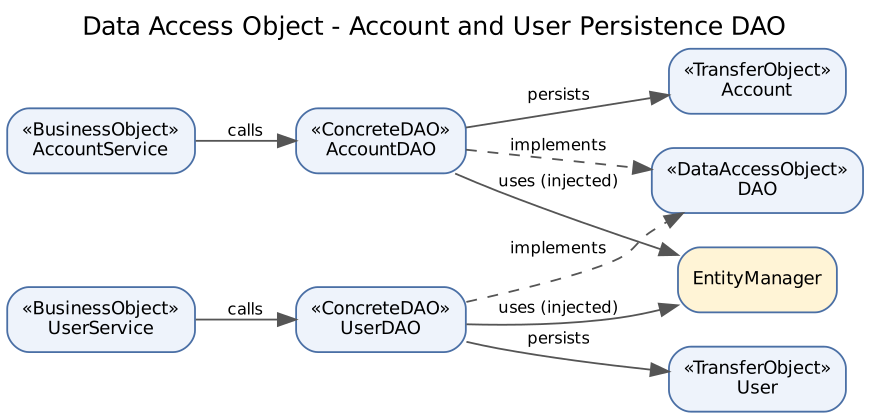
\includegraphics[width=0.86\linewidth]{Part1/pattern_architecture/instances/DAO.png}\caption{Account and User Persistence DAO -- class-level diagram (editable source \texttt{Part1/\allowbreak{}pattern\textbackslash{}\_\allowbreak{}architecture/\allowbreak{}instances/\allowbreak{}DAO.\allowbreak{}dot}).}\end{figure}
\textbf{Verification:} \textbf{Confirmed.} Reviewer: Hariprid V, Pranav R Menon, Sreyas A. Justification and tests: BaselineBehaviourTest: createUserStoresAllFields, createAccountLinksUserAndKeepsBalance, listAccountsReturnsAllAccounts (all persistence goes through the DAOs onto an in-memory EntityManager); greps C2, C6, C10. Alternatives considered: Repository (rejected as a separate instance: same collaboration, DAO naming and save/update API).
\subsubsection{API Payload DTO Assembly}
\textbf{Pattern type and category:} Data Transfer Object -- Enterprise (Fowler PoEAA / Core J2EE). \textbf{Purpose and origin:} Decouple the JSON request contract from the persistence entities and carry only the needed fields across the REST boundary. Origin: application code.
{\footnotesize
\begin{longtable}{@{}p{3.1cm}p{5.6cm}p{7cm}@{}}
\toprule \textbf{Pattern role} & \textbf{Actual class / interface / function} & \textbf{File and line range} \\ \midrule \endfirsthead
\toprule \textbf{Pattern role} & \textbf{Actual class / interface / function} & \textbf{File and line range} \\ \midrule \endhead
\bottomrule \endfoot
DataTransferObject & \texttt{UserDTO} & \texttt{persistence/\allowbreak{}dto/\allowbreak{}UserDTO.\allowbreak{}java:\allowbreak{}5-60} \\
DataTransferObject & \texttt{AccountDTO} & \texttt{persistence/\allowbreak{}dto/\allowbreak{}AccountDTO.\allowbreak{}java:\allowbreak{}6-50} \\
DataTransferObject & \texttt{TransactionDTO} & \texttt{persistence/\allowbreak{}dto/\allowbreak{}TransactionDTO.\allowbreak{}java:\allowbreak{}5-15} \\
Assembler & \texttt{UserUtil.\allowbreak{}convertToUserDTO} & \texttt{util/\allowbreak{}UserUtil.\allowbreak{}java:\allowbreak{}18-28} \\
Assembler & \texttt{AccountUtil.\allowbreak{}convertToAccount} & \texttt{util/\allowbreak{}AccountUtil.\allowbreak{}java:\allowbreak{}21-33} \\
Assembler & \texttt{UserService.\allowbreak{}createUser} & \texttt{service/\allowbreak{}UserService.\allowbreak{}java:\allowbreak{}25-34} \\
DomainObject & \texttt{User} & \texttt{persistence/\allowbreak{}model/\allowbreak{}User.\allowbreak{}java:\allowbreak{}5-56} \\
DomainObject & \texttt{Account} & \texttt{persistence/\allowbreak{}model/\allowbreak{}Account.\allowbreak{}java:\allowbreak{}5-44} \\
Consumer & \texttt{AccountController.\allowbreak{}createAccount} & \texttt{rest/\allowbreak{}AccountController.\allowbreak{}java:\allowbreak{}21-26} \\
Consumer & \texttt{AccountController.\allowbreak{}depositToAccount} & \texttt{rest/\allowbreak{}AccountController.\allowbreak{}java:\allowbreak{}28-34} \\
Consumer & \texttt{AccountController.\allowbreak{}withdraw} & \texttt{rest/\allowbreak{}AccountController.\allowbreak{}java:\allowbreak{}36-42} \\
Consumer & \texttt{UserController.\allowbreak{}createUser} & \texttt{rest/\allowbreak{}UserController.\allowbreak{}java:\allowbreak{}16-20} \\
\end{longtable}
}
\textbf{Evidence:} The three DTO classes hold fields, validation annotations and accessors only; controller methods take DTOs as parameters; convertToUserDTO, convertToAccount and UserService.createUser copy field-by-field between DTO and entity. Partial: listAccounts returns Account entities directly (output side has no DTO).
\begin{figure}[H]\centering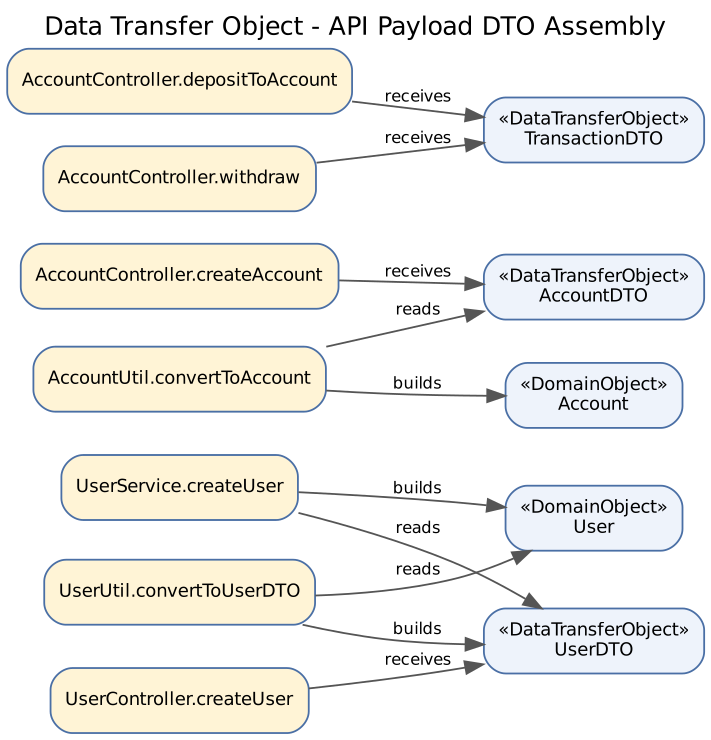
\includegraphics[width=0.86\linewidth]{Part1/pattern_architecture/instances/DTO.png}\caption{API Payload DTO Assembly -- class-level diagram (editable source \texttt{Part1/\allowbreak{}pattern\textbackslash{}\_\allowbreak{}architecture/\allowbreak{}instances/\allowbreak{}DTO.\allowbreak{}dot}).}\end{figure}
\textbf{Verification:} \textbf{Confirmed.} Reviewer: Hariprid V, Pranav R Menon, Sreyas A. Justification and tests: BaselineBehaviourTest.createUserStoresAllFields (DTO -\textgreater{} entity), deposit/withdraw tests (TransactionDTO); grep C5. Partial: listAccounts returns entities (output side not protected). Alternatives considered: Adapter / Factory for the util classes (rejected: they copy data, they do not adapt an interface or choose a product).
\subsubsection{Banking Use-Case Service Layer}
\textbf{Pattern type and category:} Service Layer -- Enterprise (Fowler PoEAA). \textbf{Purpose and origin:} Provide one application boundary that exposes the use cases and coordinates DAOs and converters for the controllers. Origin: application code.
{\footnotesize
\begin{longtable}{@{}p{3.1cm}p{5.6cm}p{7cm}@{}}
\toprule \textbf{Pattern role} & \textbf{Actual class / interface / function} & \textbf{File and line range} \\ \midrule \endfirsthead
\toprule \textbf{Pattern role} & \textbf{Actual class / interface / function} & \textbf{File and line range} \\ \midrule \endhead
\bottomrule \endfoot
ServiceLayer & \texttt{AccountService} & \texttt{service/\allowbreak{}AccountService.\allowbreak{}java:\allowbreak{}18-85} \\
ServiceLayer & \texttt{UserService} & \texttt{service/\allowbreak{}UserService.\allowbreak{}java:\allowbreak{}15-46} \\
Client & \texttt{AccountController} & \texttt{rest/\allowbreak{}AccountController.\allowbreak{}java:\allowbreak{}13-50} \\
Client & \texttt{UserController} & \texttt{rest/\allowbreak{}UserController.\allowbreak{}java:\allowbreak{}10-21} \\
Operation & \texttt{AccountService.\allowbreak{}createAccount} & \texttt{service/\allowbreak{}AccountService.\allowbreak{}java:\allowbreak{}30-34} \\
Operation & \texttt{AccountService.\allowbreak{}depositToAccount} & \texttt{service/\allowbreak{}AccountService.\allowbreak{}java:\allowbreak{}36-58} \\
Operation & \texttt{AccountService.\allowbreak{}withdraw} & \texttt{service/\allowbreak{}AccountService.\allowbreak{}java:\allowbreak{}60-79} \\
Operation & \texttt{AccountService.\allowbreak{}listAllAccounts} & \texttt{service/\allowbreak{}AccountService.\allowbreak{}java:\allowbreak{}81-83} \\
Operation & \texttt{UserService.\allowbreak{}createUser} & \texttt{service/\allowbreak{}UserService.\allowbreak{}java:\allowbreak{}25-34} \\
Operation & \texttt{UserService.\allowbreak{}getUserDetails} & \texttt{service/\allowbreak{}UserService.\allowbreak{}java:\allowbreak{}36-44} \\
Collaborator & \texttt{AccountService.\allowbreak{}accountDAO} & \texttt{service/\allowbreak{}AccountService.\allowbreak{}java:\allowbreak{}20-21} \\
Collaborator & \texttt{AccountService.\allowbreak{}userService} & \texttt{service/\allowbreak{}AccountService.\allowbreak{}java:\allowbreak{}23-24} \\
Collaborator & \texttt{AccountService.\allowbreak{}accountUtil} & \texttt{service/\allowbreak{}AccountService.\allowbreak{}java:\allowbreak{}26-27} \\
Collaborator & \texttt{UserService.\allowbreak{}userDAO} & \texttt{service/\allowbreak{}UserService.\allowbreak{}java:\allowbreak{}18-19} \\
Collaborator & \texttt{UserService.\allowbreak{}userUtil} & \texttt{service/\allowbreak{}UserService.\allowbreak{}java:\allowbreak{}21-22} \\
\end{longtable}
}
\textbf{Evidence:} Controllers call only AccountService/UserService; AccountService.createAccount coordinates userService.getUserDetails, accountUtil.convertToAccount and accountDAO.save. Deviation: transaction demarcation is on DAO methods, not on the service operations.
\begin{figure}[H]\centering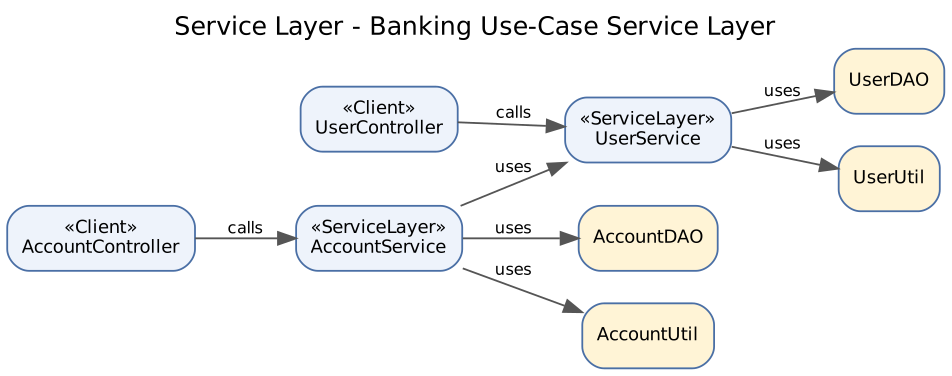
\includegraphics[width=0.86\linewidth]{Part1/pattern_architecture/instances/SL.png}\caption{Banking Use-Case Service Layer -- class-level diagram (editable source \texttt{Part1/\allowbreak{}pattern\textbackslash{}\_\allowbreak{}architecture/\allowbreak{}instances/\allowbreak{}SL.\allowbreak{}dot}).}\end{figure}
\textbf{Verification:} \textbf{Confirmed.} Reviewer: Hariprid V, Pranav R Menon, Sreyas A. Justification and tests: All BaselineBehaviourTest flows run controller -\textgreater{} service -\textgreater{} DAO; grep C5. Alternatives considered: Facade for AccountService.createAccount (uncertain: ordinary service job already counted here).
\subsubsection{Account Deposit and Withdrawal Script}
\textbf{Pattern type and category:} Transaction Script -- Enterprise (Fowler PoEAA). \textbf{Purpose and origin:} Implement each use case as one procedure that applies the business rules directly to row-like data. Origin: application code.
{\footnotesize
\begin{longtable}{@{}p{3.1cm}p{5.6cm}p{7cm}@{}}
\toprule \textbf{Pattern role} & \textbf{Actual class / interface / function} & \textbf{File and line range} \\ \midrule \endfirsthead
\toprule \textbf{Pattern role} & \textbf{Actual class / interface / function} & \textbf{File and line range} \\ \midrule \endhead
\bottomrule \endfoot
TransactionScript & \texttt{AccountService.\allowbreak{}depositToAccount} & \texttt{service/\allowbreak{}AccountService.\allowbreak{}java:\allowbreak{}36-58} \\
TransactionScript & \texttt{AccountService.\allowbreak{}withdraw} & \texttt{service/\allowbreak{}AccountService.\allowbreak{}java:\allowbreak{}60-79} \\
TransactionScript & \texttt{AccountService.\allowbreak{}createAccount} & \texttt{service/\allowbreak{}AccountService.\allowbreak{}java:\allowbreak{}30-34} \\
TransactionScript & \texttt{UserService.\allowbreak{}createUser} & \texttt{service/\allowbreak{}UserService.\allowbreak{}java:\allowbreak{}25-34} \\
RowData & \texttt{Account} & \texttt{persistence/\allowbreak{}model/\allowbreak{}Account.\allowbreak{}java:\allowbreak{}5-44} \\
\end{longtable}
}
\textbf{Evidence:} Rules are inline in the service methods: amount \textgreater{} 0 (AccountService line 43), savings bonus += 0.5 (lines 46-48), withdraw allowed only if amount \textgreater{} 0 \&\& balance \textgreater{} amount (line 67). Account contains only accessors (grep C9), i.e. an anemic entity.
\begin{figure}[H]\centering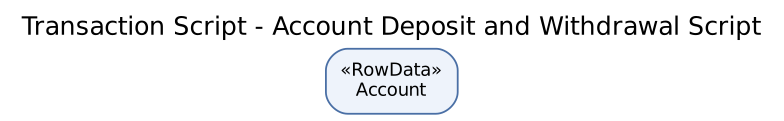
\includegraphics[width=0.86\linewidth]{Part1/pattern_architecture/instances/TS.png}\caption{Account Deposit and Withdrawal Script -- class-level diagram (editable source \texttt{Part1/\allowbreak{}pattern\textbackslash{}\_\allowbreak{}architecture/\allowbreak{}instances/\allowbreak{}TS.\allowbreak{}dot}).}\end{figure}
\textbf{Verification:} \textbf{Confirmed.} Reviewer: Hariprid V, Pranav R Menon, Sreyas A. Justification and tests: depositToSavingsAddsAmountPlusHalfBonus and withdrawOfExactlyTheBalanceIsRejectedInBaseline pin the rules that live in the service; greps C8, C9 (Account has accessors only). Alternatives considered: Domain Model (absent at baseline because Account has no behaviour; introduced in CH03).
\subsubsection{REST Use-Case Controller}
\textbf{Pattern type and category:} Controller -- GRASP. \textbf{Purpose and origin:} Receive HTTP system events and hand them to the business layer without business logic in the HTTP layer. Origin: application code.
{\footnotesize
\begin{longtable}{@{}p{3.1cm}p{5.6cm}p{7cm}@{}}
\toprule \textbf{Pattern role} & \textbf{Actual class / interface / function} & \textbf{File and line range} \\ \midrule \endfirsthead
\toprule \textbf{Pattern role} & \textbf{Actual class / interface / function} & \textbf{File and line range} \\ \midrule \endhead
\bottomrule \endfoot
Controller & \texttt{AccountController} & \texttt{rest/\allowbreak{}AccountController.\allowbreak{}java:\allowbreak{}13-50} \\
Controller & \texttt{UserController} & \texttt{rest/\allowbreak{}UserController.\allowbreak{}java:\allowbreak{}10-21} \\
SystemOperation & \texttt{AccountController.\allowbreak{}createAccount} & \texttt{rest/\allowbreak{}AccountController.\allowbreak{}java:\allowbreak{}21-26} \\
SystemOperation & \texttt{AccountController.\allowbreak{}depositToAccount} & \texttt{rest/\allowbreak{}AccountController.\allowbreak{}java:\allowbreak{}28-34} \\
SystemOperation & \texttt{AccountController.\allowbreak{}withdraw} & \texttt{rest/\allowbreak{}AccountController.\allowbreak{}java:\allowbreak{}36-42} \\
SystemOperation & \texttt{AccountController.\allowbreak{}listAccounts} & \texttt{rest/\allowbreak{}AccountController.\allowbreak{}java:\allowbreak{}44-48} \\
SystemOperation & \texttt{UserController.\allowbreak{}createUser} & \texttt{rest/\allowbreak{}UserController.\allowbreak{}java:\allowbreak{}16-20} \\
Delegate & \texttt{AccountController.\allowbreak{}accountService} & \texttt{rest/\allowbreak{}AccountController.\allowbreak{}java:\allowbreak{}16-17} \\
Delegate & \texttt{UserController.\allowbreak{}userService} & \texttt{rest/\allowbreak{}UserController.\allowbreak{}java:\allowbreak{}13-14} \\
\end{longtable}
}
\textbf{Evidence:} Each controller method unwraps the DTO, makes exactly one service call and wraps the result in a Response (grep C5); no DAO or EntityManager reference in rest/ (grep C1).
\begin{figure}[H]\centering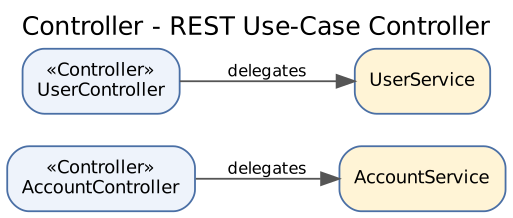
\includegraphics[width=0.86\linewidth]{Part1/pattern_architecture/instances/CTRL.png}\caption{REST Use-Case Controller -- class-level diagram (editable source \texttt{Part1/\allowbreak{}pattern\textbackslash{}\_\allowbreak{}architecture/\allowbreak{}instances/\allowbreak{}CTRL.\allowbreak{}dot}).}\end{figure}
\textbf{Verification:} \textbf{Confirmed.} Reviewer: Hariprid V, Pranav R Menon, Sreyas A. Justification and tests: createAccountEndpointReturns201, listAccountsReturnsAllAccounts; greps C1, C5, C12. Alternatives considered: Front Controller (rejected: no dispatcher code in the application).
\subsubsection{CDI Field Injection Wiring}
\textbf{Pattern type and category:} Dependency Injection -- Framework idiom (CDI / IoC). \textbf{Purpose and origin:} Let the container create and wire collaborators so that classes depend on types, not on construction. Origin: framework idiom (Jakarta CDI / Quarkus ArC) used by the application.
{\footnotesize
\begin{longtable}{@{}p{3.1cm}p{5.6cm}p{7cm}@{}}
\toprule \textbf{Pattern role} & \textbf{Actual class / interface / function} & \textbf{File and line range} \\ \midrule \endfirsthead
\toprule \textbf{Pattern role} & \textbf{Actual class / interface / function} & \textbf{File and line range} \\ \midrule \endhead
\bottomrule \endfoot
Container & (Quarkus ArC CDI container - dependency, not in application source) & not in application source \\
InjectionPoint & \texttt{AccountController.\allowbreak{}accountService} & \texttt{rest/\allowbreak{}AccountController.\allowbreak{}java:\allowbreak{}16-17} \\
InjectionPoint & \texttt{UserController.\allowbreak{}userService} & \texttt{rest/\allowbreak{}UserController.\allowbreak{}java:\allowbreak{}13-14} \\
InjectionPoint & \texttt{AccountService.\allowbreak{}accountDAO} & \texttt{service/\allowbreak{}AccountService.\allowbreak{}java:\allowbreak{}20-21} \\
InjectionPoint & \texttt{AccountService.\allowbreak{}userService} & \texttt{service/\allowbreak{}AccountService.\allowbreak{}java:\allowbreak{}23-24} \\
InjectionPoint & \texttt{AccountService.\allowbreak{}accountUtil} & \texttt{service/\allowbreak{}AccountService.\allowbreak{}java:\allowbreak{}26-27} \\
InjectionPoint & \texttt{UserService.\allowbreak{}userDAO} & \texttt{service/\allowbreak{}UserService.\allowbreak{}java:\allowbreak{}18-19} \\
InjectionPoint & \texttt{UserService.\allowbreak{}userUtil} & \texttt{service/\allowbreak{}UserService.\allowbreak{}java:\allowbreak{}21-22} \\
InjectionPoint & \texttt{AccountDAO.\allowbreak{}entityManager} & \texttt{persistence/\allowbreak{}dao/\allowbreak{}AccountDAO.\allowbreak{}java:\allowbreak{}16-17} \\
InjectionPoint & \texttt{UserDAO.\allowbreak{}entityManager} & \texttt{persistence/\allowbreak{}dao/\allowbreak{}UserDAO.\allowbreak{}java:\allowbreak{}16-17} \\
InjectionPoint & \texttt{AccountUtil.\allowbreak{}accountDAO} & \texttt{util/\allowbreak{}AccountUtil.\allowbreak{}java:\allowbreak{}17-18} \\
InjectionPoint & \texttt{UserUtil.\allowbreak{}userDAO} & \texttt{util/\allowbreak{}UserUtil.\allowbreak{}java:\allowbreak{}14-15} \\
ManagedBean & \texttt{AccountController} & \texttt{rest/\allowbreak{}AccountController.\allowbreak{}java:\allowbreak{}13-50} \\
ManagedBean & \texttt{UserController} & \texttt{rest/\allowbreak{}UserController.\allowbreak{}java:\allowbreak{}10-21} \\
ManagedBean & \texttt{AccountService} & \texttt{service/\allowbreak{}AccountService.\allowbreak{}java:\allowbreak{}18-85} \\
ManagedBean & \texttt{UserService} & \texttt{service/\allowbreak{}UserService.\allowbreak{}java:\allowbreak{}15-46} \\
ManagedBean & \texttt{AccountUtil} & \texttt{util/\allowbreak{}AccountUtil.\allowbreak{}java:\allowbreak{}14-35} \\
ManagedBean & \texttt{UserUtil} & \texttt{util/\allowbreak{}UserUtil.\allowbreak{}java:\allowbreak{}12-30} \\
ManagedBean & \texttt{AccountDAO} & \texttt{persistence/\allowbreak{}dao/\allowbreak{}AccountDAO.\allowbreak{}java:\allowbreak{}13-45} \\
ManagedBean & \texttt{UserDAO} & \texttt{persistence/\allowbreak{}dao/\allowbreak{}UserDAO.\allowbreak{}java:\allowbreak{}13-38} \\
\end{longtable}
}
\textbf{Evidence:} No collaborator is created with new (grep C3 lists only data objects and exceptions); every collaborator is an @Inject field; the unit tests build the same classes in a MiniContainer and inject an in-memory EntityManager without changing production code. Dead injection points: AccountUtil.accountDAO and UserUtil.userDAO are never used (grep C4).
\begin{figure}[H]\centering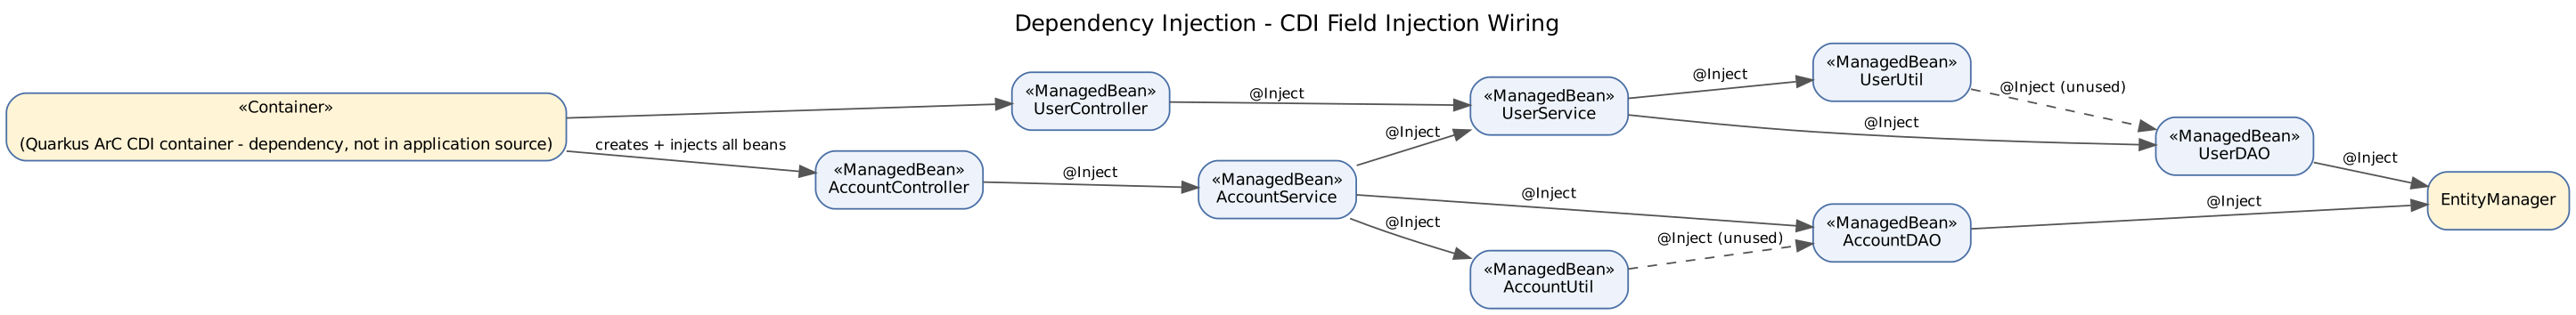
\includegraphics[width=0.86\linewidth]{Part1/pattern_architecture/instances/DI.png}\caption{CDI Field Injection Wiring -- class-level diagram (editable source \texttt{Part1/\allowbreak{}pattern\textbackslash{}\_\allowbreak{}architecture/\allowbreak{}instances/\allowbreak{}DI.\allowbreak{}dot}).}\end{figure}
\textbf{Verification:} \textbf{Confirmed.} Reviewer: Hariprid V, Pranav R Menon, Sreyas A. Justification and tests: Every test builds the real classes in a MiniContainer that injects the in-memory EntityManager into the DAOs without changing production code; greps C3, C4. Alternatives considered: GoF Singleton for the @ApplicationScoped beans (rejected: no private constructor or static instance).
\subsubsection{HTTP Error Translation}
\textbf{Pattern type and category:} Exception Translation -- Framework idiom (JAX-RS). \textbf{Purpose and origin:} Convert business failures into HTTP 400/404 responses with a message body. Origin: framework idiom (JAX-RS) used by the application.
{\footnotesize
\begin{longtable}{@{}p{3.1cm}p{5.6cm}p{7cm}@{}}
\toprule \textbf{Pattern role} & \textbf{Actual class / interface / function} & \textbf{File and line range} \\ \midrule \endfirsthead
\toprule \textbf{Pattern role} & \textbf{Actual class / interface / function} & \textbf{File and line range} \\ \midrule \endhead
\bottomrule \endfoot
TranslatedException & \texttt{BadRequestException} & \texttt{exception/\allowbreak{}BadRequestException.\allowbreak{}java:\allowbreak{}6-11} \\
TranslatedException & \texttt{NotFoundException} & \texttt{exception/\allowbreak{}NotFoundException.\allowbreak{}java:\allowbreak{}6-11} \\
Raiser & \texttt{AccountService.\allowbreak{}depositToAccount} & \texttt{service/\allowbreak{}AccountService.\allowbreak{}java:\allowbreak{}36-58} \\
Raiser & \texttt{AccountService.\allowbreak{}withdraw} & \texttt{service/\allowbreak{}AccountService.\allowbreak{}java:\allowbreak{}60-79} \\
Raiser & \texttt{AccountDAO.\allowbreak{}findById} & \texttt{persistence/\allowbreak{}dao/\allowbreak{}AccountDAO.\allowbreak{}java:\allowbreak{}19-28} \\
Raiser & \texttt{UserService.\allowbreak{}getUserDetails} & \texttt{service/\allowbreak{}UserService.\allowbreak{}java:\allowbreak{}36-44} \\
Translator & (JAX-RS runtime - dependency, not in application source) & not in application source \\
\end{longtable}
}
\textbf{Evidence:} Both exceptions extend WebApplicationException and build Response(status, message) in the constructor; service/DAO code throws them; unit tests assert getResponse().getStatus() 400/404 and the entity text. The runtime half (JAX-RS turning the exception into the HTTP reply) is framework behaviour and was not executed in the sandbox.
\begin{figure}[H]\centering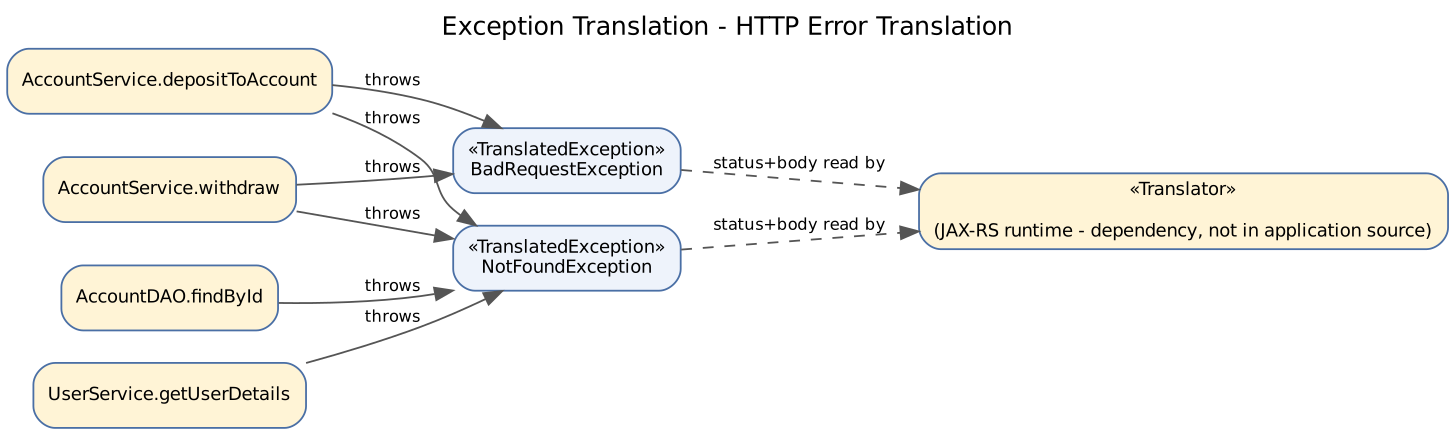
\includegraphics[width=0.86\linewidth]{Part1/pattern_architecture/instances/ET.png}\caption{HTTP Error Translation -- class-level diagram (editable source \texttt{Part1/\allowbreak{}pattern\textbackslash{}\_\allowbreak{}architecture/\allowbreak{}instances/\allowbreak{}ET.\allowbreak{}dot}).}\end{figure}
\textbf{Verification:} \textbf{Confirmed.} Reviewer: Hariprid V, Pranav R Menon, Sreyas A. Justification and tests: errorsAreCarriedAsHttpResponsesByTheCustomExceptions and the 400/404 assertions in the deposit/withdraw tests. The runtime half (JAX-RS mapping the exception to the HTTP reply) is specified by Jakarta REST but was not executed here. Alternatives considered: A separate ExceptionMapper (none exists in the application; the response is embedded in the exception).
\section{Part 2: Pattern evolution}
Three business changes were implemented one after another on the real code (git history in the local working repository; every change has a patch, a requirement file, acceptance criteria and a test log). Versions: Original = \texttt{baa96db} (+ \texttt{c9d7097} test scaffolding, production code unchanged); Change~1 = \texttt{6bdf74e}; Change~2 = \texttt{c755d20}; Change~3 = \texttt{b8de930}. Each version is counted separately, and instances \emph{replaced} by a change are excluded from the totals of the later version.
\subsection{Counts per source version}
{\footnotesize
\begin{center}\begin{tabular}{@{}p{2.7cm}ccccccccc@{}}
\toprule \textbf{Version} & \textbf{Types} & \textbf{Inst.} & \textbf{Concr.} & \textbf{Symb.} & \textbf{Fields} & \textbf{Rej./Unc.} & \textbf{NLOC} & \textbf{Files} & \textbf{Tests} \\ \midrule
Original code & 7 & 7 & 21 & 36 & 11 & 10/3 & 458 & 17 & not\_run \\
After Change1 & 8 & 8 & 24 & 41 & 12 & 10/3 & 508 & 21 & 23/23 \\
After Change2 & 9 & 9 & 28 & 48 & 14 & 11/3 & 586 & 25 & 30/30 \\
After Change3 & 9 & 9 & 28 & 56 & 14 & 12/3 & 638 & 26 & 37/37 \\
\bottomrule\end{tabular}\end{center}
}
Symbols = unique class/interface/method symbols; Fields = injection-point fields mapped additionally; Rej./Unc. = rejected/uncertain candidates in that version; NLOC and files = production code (lizard 1.24.1; maximum cyclomatic number of any function is 5 in all versions, so complexity did not grow); Tests = passing tests of the sandbox harness (the baseline column was not run in its own commit; its 15 characterization tests were added in \texttt{c9d7097} and pass on the unchanged production code).
\subsection{CH01 - Account-type policies (overdraft for checking, exact-balance withdrawal)}
\textbf{Requirement.} Business requirement: deposit bonus and withdrawal limits must depend on the account type, and a checking account may go into overdraft.\\ - Savings (CONTA\_POUPANCA): deposits still receive the 0.5 bonus; withdrawal allowed only while amount \textless{}= balance (the original code rejected a withdrawal of exactly the balance - this boundary is changed on purpose).\\ - Checking (CONTA\_CORRENTE): no bonus; withdrawal allowed while balance - amount \textgreater{}= -500.00 (overdraft limit).\\ - Amounts \textless{}= 0 are still rejected with HTTP 400; unknown accounts still 404.
{\footnotesize
\begin{longtable}{@{}p{1cm}p{7.6cm}p{7cm}@{}}
\toprule \textbf{AC} & \textbf{Acceptance criterion} & \textbf{Test} \\ \midrule \endfirsthead
\toprule \textbf{AC} & \textbf{Acceptance criterion} & \textbf{Test} \\ \midrule \endhead
\bottomrule \endfoot
AC1 & Checking with balance 100: withdraw 600 succeeds, balance becomes -500 & \texttt{Change1PolicyTest.\allowbreak{}ac1CheckingMayOverdrawUpToTheLimit} \\
AC2 & Checking with balance 100: withdraw 600.01 -\textgreater{} 400, balance unchanged & \texttt{Change1PolicyTest.\allowbreak{}ac2CheckingCannotOverdrawBeyondTheLimit} \\
AC3 & Savings with balance 100: withdraw 100.01 -\textgreater{} 400, balance unchanged & \texttt{Change1PolicyTest.\allowbreak{}ac3SavingsCannotOverdraw} \\
AC4 & Savings with balance 100: withdraw 100 succeeds, balance 0 & \texttt{Change1PolicyTest.\allowbreak{}ac4SavingsMayWithdrawExactlyTheBalance} \\
AC5 & Deposit of 5 gives +5.5 on savings and +5 on checking & \texttt{Change1PolicyTest.\allowbreak{}ac5SavingsDepositBonusIsPreservedAndCheckingHasNone} \\
AC6 & Withdrawal of 0 or negative -\textgreater{} 400 for both types & \texttt{Change1PolicyTest.\allowbreak{}ac6NonPositiveWithdrawalStillRejectedForBothTypes} \\
AC7 & Resolver returns the matching strategy; missing type -\textgreater{} 400; strategies interchangeable & \texttt{Change1PolicyTest.\allowbreak{}resolverReturnsTheMatchingStrategyAndRejectsMissingType /\allowbreak{} policiesAreInterchangeableBehindTheInterface} \\
\end{longtable}
}
\textbf{Design smell / driver.} Conditional on a type code with a magic number: AccountService.depositToAccount tested account.getType() == CONTA\_POUPANCA and added the literal 0.5; the withdrawal rule balance \textgreater{} amount was one hard-coded rule for every type, so adding the overdraft would have added more type conditionals in two methods. \textbf{Technique.} Replace Conditional with Polymorphism (Replace Type Code with Strategy): extract interface AccountPolicy, move each branch into SavingsAccountPolicy / CheckingAccountPolicy, select through AccountPolicyResolver; Replace Magic Number with Constant (DEPOSIT\_BONUS, OVERDRAFT\_LIMIT).
\textbf{Pattern effects.}
{\footnotesize
\begin{longtable}{@{}p{5.2cm}p{2.4cm}p{8cm}@{}}
\toprule \textbf{Pattern instance} & \textbf{Status} & \textbf{Note} \\ \midrule \endfirsthead
\toprule \textbf{Pattern instance} & \textbf{Status} & \textbf{Note} \\ \midrule \endhead
\bottomrule \endfoot
Strategy: Account Type Policy & newly\_introduced & Replaces the baseline conditional that was rejected as a Strategy candidate (AccountService savings-bonus if). \\
Transaction Script: Account Deposit and Withdrawal Script & modified & Still procedural, but its type-specific rules are delegated to the strategy. \\
Service Layer: Banking Use-Case Service Layer & modified & New collaborator policyResolver. \\
Dependency Injection: CDI Field Injection Wiring & extended & New bean AccountPolicyResolver and injection point. \\
DAO, DTO, Controller, Exception Translation & preserved & No participant changed. \\
\end{longtable}
}
\textbf{Behaviour preservation.} Tests: 14 of the 15 original characterization tests pass unchanged. The one that pinned the old boundary (withdrawOfExactlyTheBalanceIsRejectedInBaseline) was changed on purpose to withdrawOfExactlyTheBalanceIsAllowedAfterCh01 because AC4 changes that behaviour; savings deposit bonus, error codes and messages are covered by unchanged tests.
\begin{figure}[H]\centering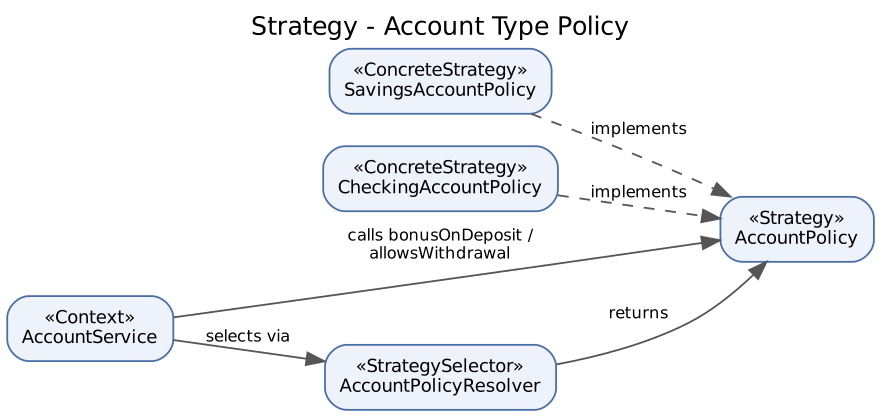
\includegraphics[width=0.8\linewidth]{Part2/diagrams/after_change1/STRAT.png}\caption{New pattern instance introduced by Change 1 (source: Part2/diagrams/after\_change1/STRAT.dot).}\end{figure}
\subsection{CH02 - Transaction events: audit log and high-value alert observers}
\textbf{Requirement.} Business requirement: every completed deposit or withdrawal must be recorded in an audit trail that can be read per account, and transactions of 10,000.00 or more must raise an alert, without the account service depending on the audit/alert code.\\ - AccountService publishes a TransactionEvent (account id, kind DEPOSIT/WITHDRAWAL, amount, balance after, timestamp) after the balance is saved.\\ - TransactionAuditLog stores events per account in order; GET /api/v1/accounts/\{id\}/audit returns them (404 for an unknown account).\\ - HighValueAlertObserver records and logs events with amount \textgreater{}= 10,000.00.\\ - Rejected operations (400/404) publish nothing.
{\footnotesize
\begin{longtable}{@{}p{1cm}p{7.6cm}p{7cm}@{}}
\toprule \textbf{AC} & \textbf{Acceptance criterion} & \textbf{Test} \\ \midrule \endfirsthead
\toprule \textbf{AC} & \textbf{Acceptance criterion} & \textbf{Test} \\ \midrule \endhead
\bottomrule \endfoot
AC1 & Deposit of 25 on balance 100 publishes one DEPOSIT event with balanceAfter 125 & \texttt{Change2ObserverTest.\allowbreak{}ac1DepositPublishesOneEventWithTheResultingBalance} \\
AC2 & Withdrawal publishes a WITHDRAWAL event & \texttt{Change2ObserverTest.\allowbreak{}ac2WithdrawalPublishesAWithdrawalEvent} \\
AC3 & Failed deposit/withdraw/unknown account publish nothing & \texttt{Change2ObserverTest.\allowbreak{}ac3FailedOperationsPublishNothing} \\
AC4 & Audit trail is per account and chronological & \texttt{Change2ObserverTest.\allowbreak{}ac4AuditTrailIsPerAccountAndChronological} \\
AC5 & Audit endpoint returns 200 + trail; 404 for an unknown account & \texttt{Change2ObserverTest.\allowbreak{}ac5AuditEndpointReturnsTheTrailAndNotFoundForUnknownAccount} \\
AC6 & Alert raised at exactly 10000.00, not at 9999.99 & \texttt{Change2ObserverTest.\allowbreak{}ac6HighValueTransactionsRaiseAnAlertAtTheThreshold} \\
AC7 & AccountService holds no reference to a concrete observer & \texttt{Change2ObserverTest.\allowbreak{}ac7AccountServiceKnowsNoConcreteObserver} \\
\end{longtable}
}
\textbf{Design smell / driver.} Preventive: audit and alerting would otherwise be written as direct calls inside depositToAccount/withdraw, giving the service a new dependency (and a new edit) for every reaction (Divergent Change / Shotgun Surgery risk). No existing smell was removed in this change. \textbf{Technique.} Replace direct calls with publish/subscribe (introduce Observer through CDI events); the event is an immutable record.
\textbf{Pattern effects.}
{\footnotesize
\begin{longtable}{@{}p{5.2cm}p{2.4cm}p{8cm}@{}}
\toprule \textbf{Pattern instance} & \textbf{Status} & \textbf{Note} \\ \midrule \endfirsthead
\toprule \textbf{Pattern instance} & \textbf{Status} & \textbf{Note} \\ \midrule \endhead
\bottomrule \endfoot
Observer: Transaction Audit and Alert Notification & newly\_introduced & New event type, two concrete observers; AccountService is the subject (CDI Event). \\
Transaction Script & modified & deposit/withdraw also fire an event. \\
Service Layer & extended & New use case getAuditTrail. \\
Controller & extended & New system operation listAudit. \\
Dependency Injection & extended & Event\textless{}TransactionEvent\textgreater{}, TransactionAuditLog injected; two observer beans. \\
Strategy, DAO, DTO, Exception Translation & preserved & No participant changed. \\
\end{longtable}
}
\textbf{Behaviour preservation.} Tests: all 23 tests of the previous version pass unchanged (30/30 in total); the only edits to existing test code are two additional beans registered in TestApp. Balances and HTTP statuses of deposit/withdraw are unchanged.
\begin{figure}[H]\centering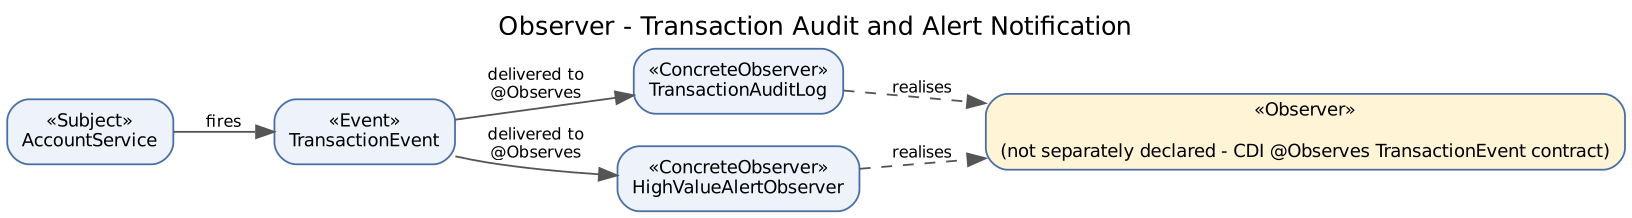
\includegraphics[width=0.8\linewidth]{Part2/diagrams/after_change2/OBS.png}\caption{New pattern instance introduced by Change 2 (source: Part2/diagrams/after\_change2/OBS.dot).}\end{figure}
\subsection{CH03 - Atomic funds transfer; business rules move into Account}
\textbf{Requirement.} Business requirement: customers can transfer money between two accounts atomically.\\ - POST /api/v1/accounts/transfer with fromAccountId, toAccountId, amount.\\ - The source account applies its own policy (overdraft for checking, none for savings); the target is credited without the savings deposit bonus.\\ - Same account, missing ids and amount \textless{}= 0 -\textgreater{} 400; unknown account -\textgreater{} 404; insufficient funds -\textgreater{} 400. In every failure neither account changes.\\ - The operation is one transaction (service-level @Transactional) and publishes TRANSFER\_OUT and TRANSFER\_IN events.\\ Refactoring that enables it: the deposit/withdraw rules move from AccountService into the Account entity so that deposit, withdraw and transfer share one implementation.
{\footnotesize
\begin{longtable}{@{}p{1cm}p{7.6cm}p{7cm}@{}}
\toprule \textbf{AC} & \textbf{Acceptance criterion} & \textbf{Test} \\ \midrule \endfirsthead
\toprule \textbf{AC} & \textbf{Acceptance criterion} & \textbf{Test} \\ \midrule \endhead
\bottomrule \endfoot
AC1 & Transfer 30 from checking(100) to savings(50): 70 and 80 (no bonus) & \texttt{Change3TransferTest.\allowbreak{}ac1TransferMovesTheAmountWithoutDepositBonus} \\
AC2 & Insufficient funds on savings source -\textgreater{} 400, both balances unchanged & \texttt{Change3TransferTest.\allowbreak{}ac2InsufficientFundsChangesNeitherAccount} \\
AC3 & Checking source may use its overdraft (-500 / 650) & \texttt{Change3TransferTest.\allowbreak{}ac3CheckingSourceMayUseItsOverdraft} \\
AC4 & Same account, amount \textless{}= 0, missing id -\textgreater{} 400, nothing changes & \texttt{Change3TransferTest.\allowbreak{}ac4SameAccountAndNonPositiveAmountAndMissingIdsAreBadRequests} \\
AC5 & Unknown source or target -\textgreater{} 404, nothing changes & \texttt{Change3TransferTest.\allowbreak{}ac5UnknownAccountIsNotFoundAndNothingChanges} \\
AC6 & TRANSFER\_OUT and TRANSFER\_IN events with the new balances & \texttt{Change3TransferTest.\allowbreak{}ac6TransferPublishesOutAndInEvents} \\
AC7 & Account enforces deposit/withdraw/credit rules by itself & \texttt{Change3TransferTest.\allowbreak{}ac7AccountEnforcesItsOwnRulesWithoutTheService} \\
\end{longtable}
}
\textbf{Design smell / driver.} Anemic Domain Model / Feature Envy: AccountService read and wrote Account.balance and applied all rules while Account only had accessors; the deposit and withdraw procedures also duplicated the load-validate-save-publish shape, and contained an unreachable else-branch (AccountDAO.findById never returns an empty Optional - it throws NotFoundException - so `optionalAccount != null \&\& isPresent()` was always true). \textbf{Technique.} Move Method (rules to Account), Extract Method (loadAccount, publish), Remove Dead Code / Replace Optional-null checks with orElseThrow.
\textbf{Pattern effects.}
{\footnotesize
\begin{longtable}{@{}p{5.2cm}p{2.4cm}p{8cm}@{}}
\toprule \textbf{Pattern instance} & \textbf{Status} & \textbf{Note} \\ \midrule \endfirsthead
\toprule \textbf{Pattern instance} & \textbf{Status} & \textbf{Note} \\ \midrule \endhead
\bottomrule \endfoot
Transaction Script: Account Deposit and Withdrawal Script & replaced & Rules moved into Account; remaining service methods are plain orchestration/CRUD. \\
Domain Model: Account Balance Domain Model & newly\_introduced & Replaces the script; Account.deposit/withdraw/credit hold the rules. \\
Strategy & modified & Context moves from AccountService to Account. \\
Observer & modified & Publishing centralised in AccountService.publish; new transfer event kinds. \\
Service Layer & modified & New transfer use case; deposit/withdraw/transfer are service-level transactions. \\
DTO & extended & TransferDTO. \\
Controller & extended & transfer operation. \\
Exception Translation & extended & Account and transfer raise BadRequestException; loadAccount raises NotFoundException. \\
DAO, Dependency Injection & preserved & No participant changed. \\
\end{longtable}
}
\textbf{Behaviour preservation.} Tests: all 30 tests of the previous version pass unchanged (37/37 in total) - same balances, same statuses, same messages for deposit and withdraw. Not covered by any test: rollback of a failed transfer inside a real database transaction (requires Quarkus + a database; see README).
\begin{figure}[H]\centering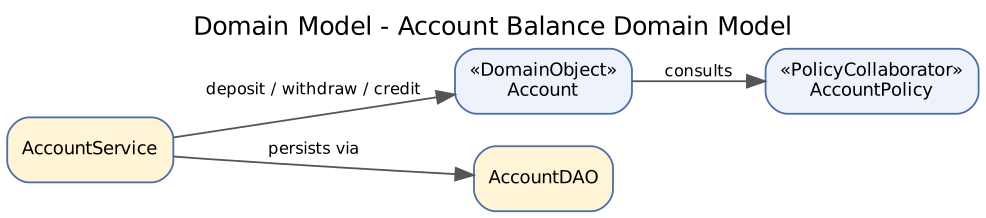
\includegraphics[width=0.8\linewidth]{Part2/diagrams/after_change3/DM.png}\caption{New pattern instance introduced by Change 3 (source: Part2/diagrams/after\_change3/DM.dot).}\end{figure}
\subsection{Status of every instance across versions}
{\footnotesize
\begin{center}\begin{tabular}{@{}p{5.6cm}p{2.5cm}p{2.5cm}p{2.5cm}p{2.5cm}@{}}
\toprule \textbf{Instance} & \textbf{Orig.} & \textbf{Ch.1} & \textbf{Ch.2} & \textbf{Ch.3} \\ \midrule
Account and User Persistence DAO & baseline & preserved & preserved & preserved \\
API Payload DTO Assembly & baseline & preserved & preserved & extended \\
Banking Use-Case Service Layer & baseline & modified & extended & modified \\
Account Deposit and Withdrawal Script & baseline & modified & modified & replaced \\
REST Use-Case Controller & baseline & preserved & extended & extended \\
CDI Field Injection Wiring & baseline & extended & extended & preserved \\
HTTP Error Translation & baseline & preserved & preserved & extended \\
Account Type Policy & -- & newly\_introduced & preserved & modified \\
Transaction Audit and Alert Notification & -- & -- & newly\_introduced & modified \\
Account Balance Domain Model & -- & -- & -- & newly\_introduced \\
\bottomrule\end{tabular}\end{center}
}
\textbf{Interpretation.} The layered patterns (DAO, DTO, Service Layer, Controller, Exception Translation) were preserved through all three changes: new behaviour was added around them rather than into them. Strategy removed a type-code conditional and made the next account type an additive change. The Observer decoupled reactions from the service and cost one new dependency (event injection) in it. Moving the rules into \texttt{Account} (Domain Model) retired the Transaction Script instance, so the number of types rose 7, 8, 9 and then stayed at 9 (Domain Model in, Transaction Script out). Limitation: the claims about transaction rollback of a failed transfer and about the HTTP/JPA wiring are not verified (no Quarkus run).
\section{Part 3: Cross-language comparison}
Ten pattern instances of the final application were re-implemented as small self-contained snippets in Java, Python, JavaScript (Node) and C++, 40 snippets in total, each with a runner that executes shared test cases (\texttt{Part3/\allowbreak{}\textless{}problem\textgreater{}/\allowbreak{}test-cases/\allowbreak{}cases.\allowbreak{}txt}). The snippets are \emph{simplified, in-memory} versions: no frameworks, so CDI, JAX-RS and JPA behaviour is not exercised -- the roles and collaborations are.
\subsection{Selected instances and common specification}
{\footnotesize
\begin{center}\begin{tabular}{@{}p{3.2cm}p{5.4cm}p{5.6cm}p{1.2cm}@{}}
\toprule \textbf{Pattern} & \textbf{Instance} & \textbf{Folder} & \textbf{Cases} \\ \midrule
Data Access Object & Account and User Persistence DAO & \texttt{dao\_\allowbreak{}account\_\allowbreak{}persistence} & 7 \\
Data Transfer Object & API Payload DTO Assembly & \texttt{dto\_\allowbreak{}user\_\allowbreak{}assembly} & 5 \\
Service Layer & Banking Use-Case Service Layer & \texttt{service\_\allowbreak{}layer\_\allowbreak{}bank} & 6 \\
Transaction Script & Account Deposit and Withdrawal Script & \texttt{transaction\_\allowbreak{}script\_\allowbreak{}account} & 8 \\
Controller & REST Use-Case Controller & \texttt{controller\_\allowbreak{}rest\_\allowbreak{}use\_\allowbreak{}case} & 5 \\
Dependency Injection & CDI Field Injection Wiring & \texttt{dependency\_\allowbreak{}injection\_\allowbreak{}wiring} & 7 \\
Exception Translation & HTTP Error Translation & \texttt{exception\_\allowbreak{}translation\_\allowbreak{}http} & 6 \\
Strategy & Account Type Policy & \texttt{strategy\_\allowbreak{}account\_\allowbreak{}policy} & 8 \\
Observer & Transaction Audit and Alert Notification & \texttt{observer\_\allowbreak{}transaction\_\allowbreak{}events} & 8 \\
Domain Model & Account Balance Domain Model & \texttt{domain\_\allowbreak{}model\_\allowbreak{}account} & 12 \\
\bottomrule\end{tabular}\end{center}
}
Fixture format: \texttt{cmd1;cmd2 =\textgreater{} expected output of the last command}, numbers with two decimals; every runner prints \texttt{RESULT passed=N total=M} and the role check (\texttt{Part3/\allowbreak{}evidence/\allowbreak{}role\textbackslash{}\_\allowbreak{}check.\allowbreak{}txt}) found every declared role in all 40 snippets (duck-typed languages have recorded exemptions for interfaces).
\subsection{Results}
{\footnotesize
\begin{longtable}{@{}p{5.6cm}p{2.2cm}p{1.2cm}p{1.4cm}p{2.4cm}p{2cm}@{}}
\toprule \textbf{Instance} & \textbf{Language} & \textbf{LOC} & \textbf{Max CC} & \textbf{Tests} & \textbf{Median ms} \\ \midrule \endfirsthead
\toprule \textbf{Instance} & \textbf{Language} & \textbf{LOC} & \textbf{Max CC} & \textbf{Tests} & \textbf{Median ms} \\ \midrule \endhead
\bottomrule \endfoot
Account and User Persistence D & Java & 42 & 2 & 7/7 passed & 99.3 \\
Account and User Persistence D & Python & 33 & 2 & 7/7 passed & 18.5 \\
Account and User Persistence D & JavaScript & 29 & 2 & 7/7 passed & 49.9 \\
Account and User Persistence D & C++ & 47 & 2 & 7/7 passed & 4.2 \\
API Payload DTO Assembly & Java & 18 & 1 & 5/5 passed & 105.4 \\
API Payload DTO Assembly & Python & 15 & 1 & 5/5 passed & 16.1 \\
API Payload DTO Assembly & JavaScript & 13 & 1 & 5/5 passed & 35.2 \\
API Payload DTO Assembly & C++ & 15 & 1 & 5/5 passed & 3.8 \\
Banking Use-Case Service Layer & Java & 30 & 3 & 6/6 passed & 86.5 \\
Banking Use-Case Service Layer & Python & 32 & 2 & 6/6 passed & 22.0 \\
Banking Use-Case Service Layer & JavaScript & 25 & 2 & 6/6 passed & 34.2 \\
Banking Use-Case Service Layer & C++ & 32 & 3 & 6/6 passed & 3.2 \\
Account Deposit and Withdrawal & Java & 40 & 3 & 8/8 passed & 87.3 \\
Account Deposit and Withdrawal & Python & 33 & 3 & 8/8 passed & 17.7 \\
Account Deposit and Withdrawal & JavaScript & 26 & 3 & 8/8 passed & 36.5 \\
Account Deposit and Withdrawal & C++ & 38 & 3 & 8/8 passed & 3.8 \\
REST Use-Case Controller & Java & 19 & 1 & 5/5 passed & 124.3 \\
REST Use-Case Controller & Python & 17 & 1 & 5/5 passed & 16.3 \\
REST Use-Case Controller & JavaScript & 8 & 1 & 5/5 passed & 47.5 \\
REST Use-Case Controller & C++ & 20 & 1 & 5/5 passed & 3.2 \\
CDI Field Injection Wiring & Java & 32 & 4 & 7/7 passed & 79.2 \\
CDI Field Injection Wiring & Python & 35 & 4 & 7/7 passed & 18.4 \\
CDI Field Injection Wiring & JavaScript & 27 & 2 & 7/7 passed & 36.0 \\
CDI Field Injection Wiring & C++ & 36 & 4 & 7/7 passed & 3.1 \\
HTTP Error Translation & Java & 29 & 3 & 6/6 passed & 99.3 \\
HTTP Error Translation & Python & 27 & 3 & 6/6 passed & 14.7 \\
HTTP Error Translation & JavaScript & 24 & 3 & 6/6 passed & 33.6 \\
HTTP Error Translation & C++ & 29 & 3 & 6/6 passed & 3.1 \\
Account Type Policy & Java & 34 & 3 & 8/8 passed & 112.0 \\
Account Type Policy & Python & 35 & 3 & 8/8 passed & 16.4 \\
Account Type Policy & JavaScript & 30 & 3 & 8/8 passed & 48.6 \\
Account Type Policy & C++ & 37 & 3 & 8/8 passed & 3.4 \\
Transaction Audit and Alert No & Java & 46 & 3 & 8/8 passed & 96.4 \\
Transaction Audit and Alert No & Python & 40 & 3 & 8/8 passed & 17.4 \\
Transaction Audit and Alert No & JavaScript & 32 & 3 & 8/8 passed & 34.0 \\
Transaction Audit and Alert No & C++ & 54 & 5 & 8/8 passed & 3.0 \\
Account Balance Domain Model & Java & 43 & 4 & 12/12 passed & 96.4 \\
Account Balance Domain Model & Python & 48 & 4 & 12/12 passed & 15.7 \\
Account Balance Domain Model & JavaScript & 36 & 4 & 12/12 passed & 35.3 \\
Account Balance Domain Model & C++ & 48 & 4 & 12/12 passed & 3.9 \\
\end{longtable}
}
\textbf{Rules.} LOC = non-blank non-comment lines of the snippet (runner excluded); Max CC = highest function cyclomatic number by lizard 1.24.1. Time = median of five timed runs after one warm-up run, compiled first, measured on the whole process (JVM/interpreter start-up plus reading the fixture file, compilation excluded; raw data in \texttt{Part3/\allowbreak{}evidence/\allowbreak{}timing\textbackslash{}\_\allowbreak{}raw.\allowbreak{}csv}). Environment: shared 2-vCPU container (\texttt{machine.\allowbreak{}txt}), so the times are indicative only, not benchmarks.
\begin{figure}[H]\centering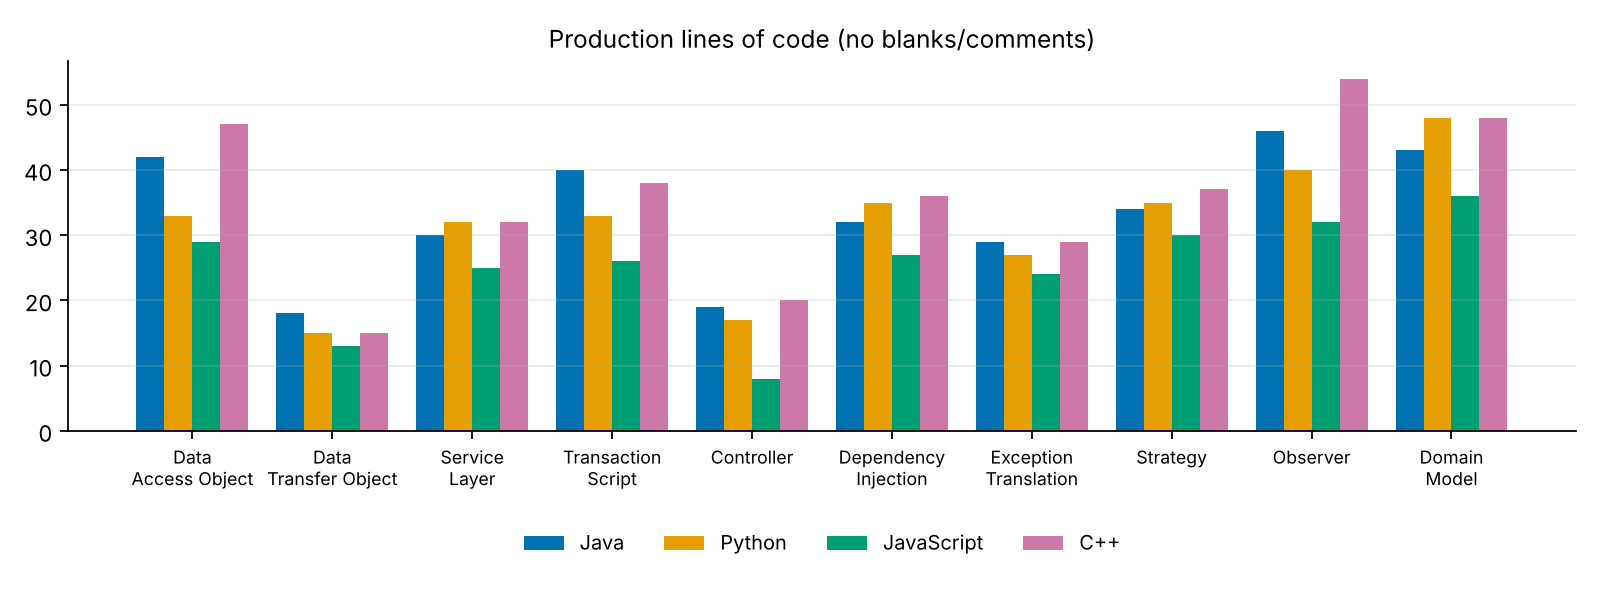
\includegraphics[width=0.85\linewidth]{Part3/evidence/charts/loc_by_language.png}\caption{Source lines of code per problem and language.}\end{figure}
\begin{figure}[H]\centering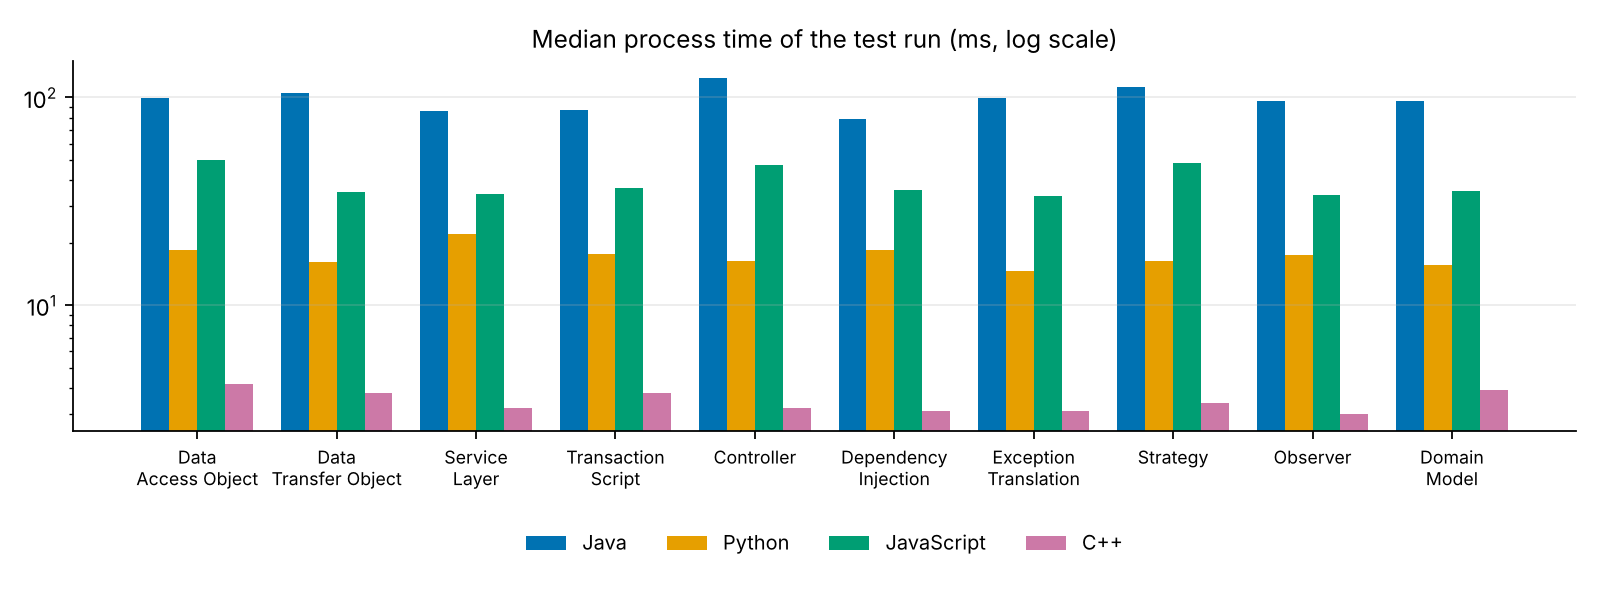
\includegraphics[width=0.85\linewidth]{Part3/evidence/charts/median_ms_by_language.png}\caption{Median process time per problem and language (log scale).}\end{figure}
{\small
\begin{center}\begin{tabular}{@{}p{3cm}p{3cm}p{3.5cm}p{3cm}@{}}
\toprule \textbf{Language} & \textbf{Median LOC} & \textbf{Median max CC} & \textbf{Median ms} \\ \midrule
Java & 33.0 & 3.0 & 97.8 \\
Python & 33.0 & 3.0 & 16.9 \\
JavaScript & 26.5 & 2.5 & 35.6 \\
C++ & 36.5 & 3.0 & 3.3 \\
\bottomrule\end{tabular}\end{center}
}
\textbf{Comparison.} Python and JavaScript snippets are the shortest because interfaces, getters and type declarations disappear (Strategy, Observer and DAO need no interface type; duck typing supplies the role). Java and C++ are longest: Java for explicit interfaces and exception classes, C++ for headers-in-file, constructors, ownership (smart pointers) and the standard-library plumbing. Cyclomatic complexity is nearly language independent, since it follows the pattern logic, not the syntax. Process time is dominated by start-up: native C++ is fastest, then Python, Node, and the JVM slowest -- this says nothing about steady-state speed. Patterns whose purpose is compensating for static typing (Strategy as an interface, Dependency Injection through a container) shrink to a function or a constructor argument in the dynamic languages, while patterns tied to a framework (Exception Translation, Controller, DI container) lose the framework and keep only the structure.
\textbf{Limitations.} The shared fixtures and the snippets come from the same LLM session (not independent); timings come from a shared container; snippets are simplified.
\section{LLM usage records}
The three prompts of each part belong to the three members. In this submission they were all run in one assistant session (Claude Sonnet 5.5, id claude-sonnet-5-5; the serving model may differ) on 2026-10-11, so the members may need to replay their own prompt in their own account if the course demands separate accounts: \ph{member-to-prompt assignment / replay confirmation}. Files named \texttt{output\textbackslash{}\_\allowbreak{}ch0N.\allowbreak{}md} are design notes written by the model; the generated code itself is the patch of each change. Every ``evaluation'' below was checked against the code or the tests, not taken from the model.
{\footnotesize
\begin{longtable}{@{}p{1.1cm}p{3cm}p{3.3cm}p{8.3cm}@{}}
\toprule \textbf{Part} & \textbf{Prompt} & \textbf{Output} & \textbf{Evaluation (verified)} \\ \midrule \endfirsthead
\toprule \textbf{Part} & \textbf{Prompt} & \textbf{Output} & \textbf{Evaluation (verified)} \\ \midrule \endhead
\bottomrule \endfoot
Part 1 & \texttt{prompt\_\allowbreak{}m1.\allowbreak{}txt} & \texttt{output\_\allowbreak{}m1.\allowbreak{}md} & Correct: 3 confirmed + 2 rejected candidates kept; all 18 file:line rows matched the source exactly and every behavioural claim passed the grep checks. \\
Part 1 & \texttt{prompt\_\allowbreak{}m2.\allowbreak{}txt} & \texttt{output\_\allowbreak{}m2.\allowbreak{}md} & Partial: all 34 file:line rows matched; one claim was wrong - it said the only 'new' expressions create data objects, but exceptions are also created with new (claims\_check C3). Corrected in the report; the DI conclusion is unaffected (no collaborator is created with new). \\
Part 1 & \texttt{prompt\_\allowbreak{}m3.\allowbreak{}txt} & \texttt{output\_\allowbreak{}m3.\allowbreak{}md} & Correct: all 16 file:line rows matched; defects (Optional.of(null), dead catch, getAll null) confirmed by grep and by tests; the 2 uncertain candidates are kept uncertain because they cannot be proven in the sandbox. \\
Part 2 & \texttt{prompt\_\allowbreak{}ch01.\allowbreak{}txt} & \texttt{output\_\allowbreak{}ch01.\allowbreak{}md} & Partial: production code compiled and all 23 tests passed on the first run, and the pattern analysis (Strategy introduced, Transaction Script modified) matches the code. One unannounced behaviour change was found in review: an account whose type is null could be credited before, but now gets HTTP 400 from AccountPolicyResolver.forType(null). One existing test had to be edited because the boundary change (AC4) was intended. \\
Part 2 & \texttt{prompt\_\allowbreak{}ch02.\allowbreak{}txt} & \texttt{output\_\allowbreak{}ch02.\allowbreak{}md} & Partial: code compiled and 30/30 tests passed on the first run; claims about event content, per-account order, 400/404 publishing nothing and the 10000.00 threshold are confirmed by tests. Cannot confirm: that the audit trail stays correct if the surrounding database transaction rolls back after the event is fired (observers run synchronously inside the transaction; needs Quarkus + a database). \\
Part 2 & \texttt{prompt\_\allowbreak{}ch03.\allowbreak{}txt} & \texttt{output\_\allowbreak{}ch03.\allowbreak{}md} & Partial: code compiled and 37/37 tests passed on the first run; the Move Method refactoring preserved all earlier test results unchanged. The claim that the transfer is atomic is confirmed only for validation failures (nothing is persisted when a rule fails); rollback after a failure between the two DAO updates relies on @Transactional and was not executed. The unreachable-else-branch finding in the old deposit/withdraw code was confirmed by reading AccountDAO.findById. \\
Part 3 & \texttt{prompt\_\allowbreak{}m1.\allowbreak{}txt} & \texttt{output\_\allowbreak{}m1\_\allowbreak{}generated\_\allowbreak{}code.\allowbreak{}txt} & Correct on execution: all 16 snippets (4 problems x 4 languages) compiled and passed 100\% of their shared cases on the first run, and the role check found every declared role. Limitations: the fixtures were written by the same model from the Java behaviour, so they are not independent of the model; the snippets are simplified (in-memory, no framework), so framework behaviour (CDI, JAX-RS, JPA) is not exercised. \\
Part 3 & \texttt{prompt\_\allowbreak{}m2.\allowbreak{}txt} & \texttt{output\_\allowbreak{}m2\_\allowbreak{}generated\_\allowbreak{}code.\allowbreak{}txt} & Correct on execution: all 12 snippets (3 problems x 4 languages) compiled and passed 100\% of their shared cases on the first run, and the role check found every declared role. Limitations: the fixtures were written by the same model from the Java behaviour, so they are not independent of the model; the snippets are simplified (in-memory, no framework), so framework behaviour (CDI, JAX-RS, JPA) is not exercised. \\
Part 3 & \texttt{prompt\_\allowbreak{}m3.\allowbreak{}txt} & \texttt{output\_\allowbreak{}m3\_\allowbreak{}generated\_\allowbreak{}code.\allowbreak{}txt} & Correct on execution: all 12 snippets (3 problems x 4 languages) compiled and passed 100\% of their shared cases on the first run, and the role check found every declared role. Limitations: the fixtures were written by the same model from the Java behaviour, so they are not independent of the model; the snippets are simplified (in-memory, no framework), so framework behaviour (CDI, JAX-RS, JPA) is not exercised. \\
\end{longtable}
}
Human reviewer sign-off: Hariprid V, Pranav R Menon, Sreyas A.
\section{Findings, contributions and references}
\subsection{Findings}
\begin{itemize}\item Pattern mix: the baseline is a conventional layered design with 7 confirmed patterns; its weakest point is that the DAO abstraction is bypassed (services inject the concrete DAOs) and the business rules sit in the service (Transaction Script, anemic entity).\end{itemize}
\begin{itemize}\item Defects found while verifying (not fixed, since they are outside the requested changes): \texttt{UserDAO.\allowbreak{}findById} can throw a NullPointerException and has a dead catch; \texttt{getAll} may return null; the Bean-Validation annotations are ineffective because the controllers lack \texttt{@Valid}; \texttt{Account} has no \texttt{getId}; the user password is stored and exposed as plain text; the template tests are stale.\end{itemize}
\begin{itemize}\item Counting: with the rule that replaced instances are excluded, types went 7, 8, 9, 9 and instances 7, 8, 9, 9; concrete classes 21, 24, 28, 28; production NLOC 458, 508, 586, 638 with maximum CC constant at 5.\end{itemize}
\begin{itemize}\item Behaviour changes made on purpose: CH01 allows withdrawing exactly the balance and returns 400 for a null account type.\end{itemize}
\begin{itemize}\item Not verified: a real Quarkus build/test run, database transactions (rollback of failed transfers) and HTTP wiring -- run \texttt{.\allowbreak{}/\allowbreak{}mvnw test} in \texttt{Part2/\allowbreak{}code} before submission.\end{itemize}
\subsection{Contributions}
{\small
\begin{center}\begin{tabular}{@{}p{4cm}p{11.6cm}@{}}
\toprule \textbf{Member} & \textbf{Contribution} \\ \midrule
Hariprid V & \ph{prompt, analysis, testing, report parts} \\
Pranav R Menon & \ph{prompt, analysis, testing, report parts} \\
Sreyas A & \ph{prompt, analysis, testing, report parts} \\
\bottomrule\end{tabular}\end{center}
}
\subsection{References}
\begin{enumerate}\item M. Fowler, \textit{Patterns of Enterprise Application Architecture}, Addison-Wesley, 2002: Transaction Script, Service Layer, Data Transfer Object, Domain Model, \url{https://martinfowler.com/eaaCatalog/}.\item Oracle, Core J2EE Patterns: Data Access Object, \url{https://www.oracle.com/java/technologies/dataaccessobject.html}.\item E. Gamma, R. Helm, R. Johnson, J. Vlissides, \textit{Design Patterns}, Addison-Wesley, 1994 (Strategy, Observer, Template Method).\item C. Larman, \textit{Applying UML and Patterns}, 3rd ed., 2004 (GRASP Controller).\item Jakarta Contexts and Dependency Injection 4.0, \url{https://jakarta.ee/specifications/cdi/4.0/jakarta-cdi-spec-4.0.html}.\item Jakarta RESTful Web Services 3.1, \url{https://jakarta.ee/specifications/restful-ws/3.1/jakarta-restful-ws-spec-3.1.html}.\item Quarkus CDI reference, \url{https://quarkus.io/guides/cdi-reference}.\item lizard code complexity analyser, \url{https://github.com/terryyin/lizard}.\end{enumerate}
\section{Team folder and repository}
Folder layout of the submission (generated listing, the large per-problem folders are summarised):
\begin{Verbatim}[fontsize=\scriptsize]
.
Part1
Part1/Part1_prompt.txt
Part1/Pattern_count.csv
Part1/evidence
Part1/llm
Part1/llm.csv
Part1/pattern_architecture
Part1/patterns.csv
Part2
Part2/Part2_prompt.txt
Part2/Pattern_count.csv
Part2/changes
Part2/code
Part2/diagrams
Part2/evidence
Part2/llm
Part2/llm.csv
Part2/pattern_evolution.csv
Part3
Part3/controller_rest_use_case
Part3/dao_account_persistence
Part3/dependency_injection_wiring
Part3/domain_model_account
Part3/dto_user_assembly
Part3/evidence
Part3/exception_translation_http
Part3/llm
Part3/observer_transaction_events
Part3/service_layer_bank
Part3/strategy_account_policy
Part3/transaction_script_account
README.md
data
data/code
data/test_result
data/test_result/README.md
data/test_result/baseline_tests
data/test_result/baseline_tests_run.log
data/test_result/harness
data/test_result/tools

\end{Verbatim}
Note on CSV placement: the two instruction PDFs disagree on whether the CSV files are repeated inside the part folders; this package keeps one copy at the place named in the explicit tree. Part~3's cross-language CSV is named \texttt{pattern\textbackslash{}\_\allowbreak{}crosslanguage.\allowbreak{}csv} as in the tree, and the Part~2 prompt file is \texttt{Part2\textbackslash{}\_\allowbreak{}prompt.\allowbreak{}txt} (the tree writes .text).
GitHub: repository \ph{URL}, screenshots of the commit history and folder view: \ph{screenshots}
\end{document}
